\documentclass[12pt]{article}

\usepackage[spanish]{babel}
\usepackage[utf8]{inputenc}
\usepackage{graphicx}
\usepackage{geometry}
\usepackage{xcolor}
\usepackage{fancyhdr}
\usepackage{lastpage}
\usepackage{pdfpages}
\usepackage{listings}

\geometry{top=25mm,left=15mm,right=15mm,a4paper}

\pagestyle{fancy}
\fancyhf{}
\lhead{Lenguajes de Programación}
\cfoot{Página \thepage\ de \pageref{LastPage}}

\graphicspath{./}

\begin{document}
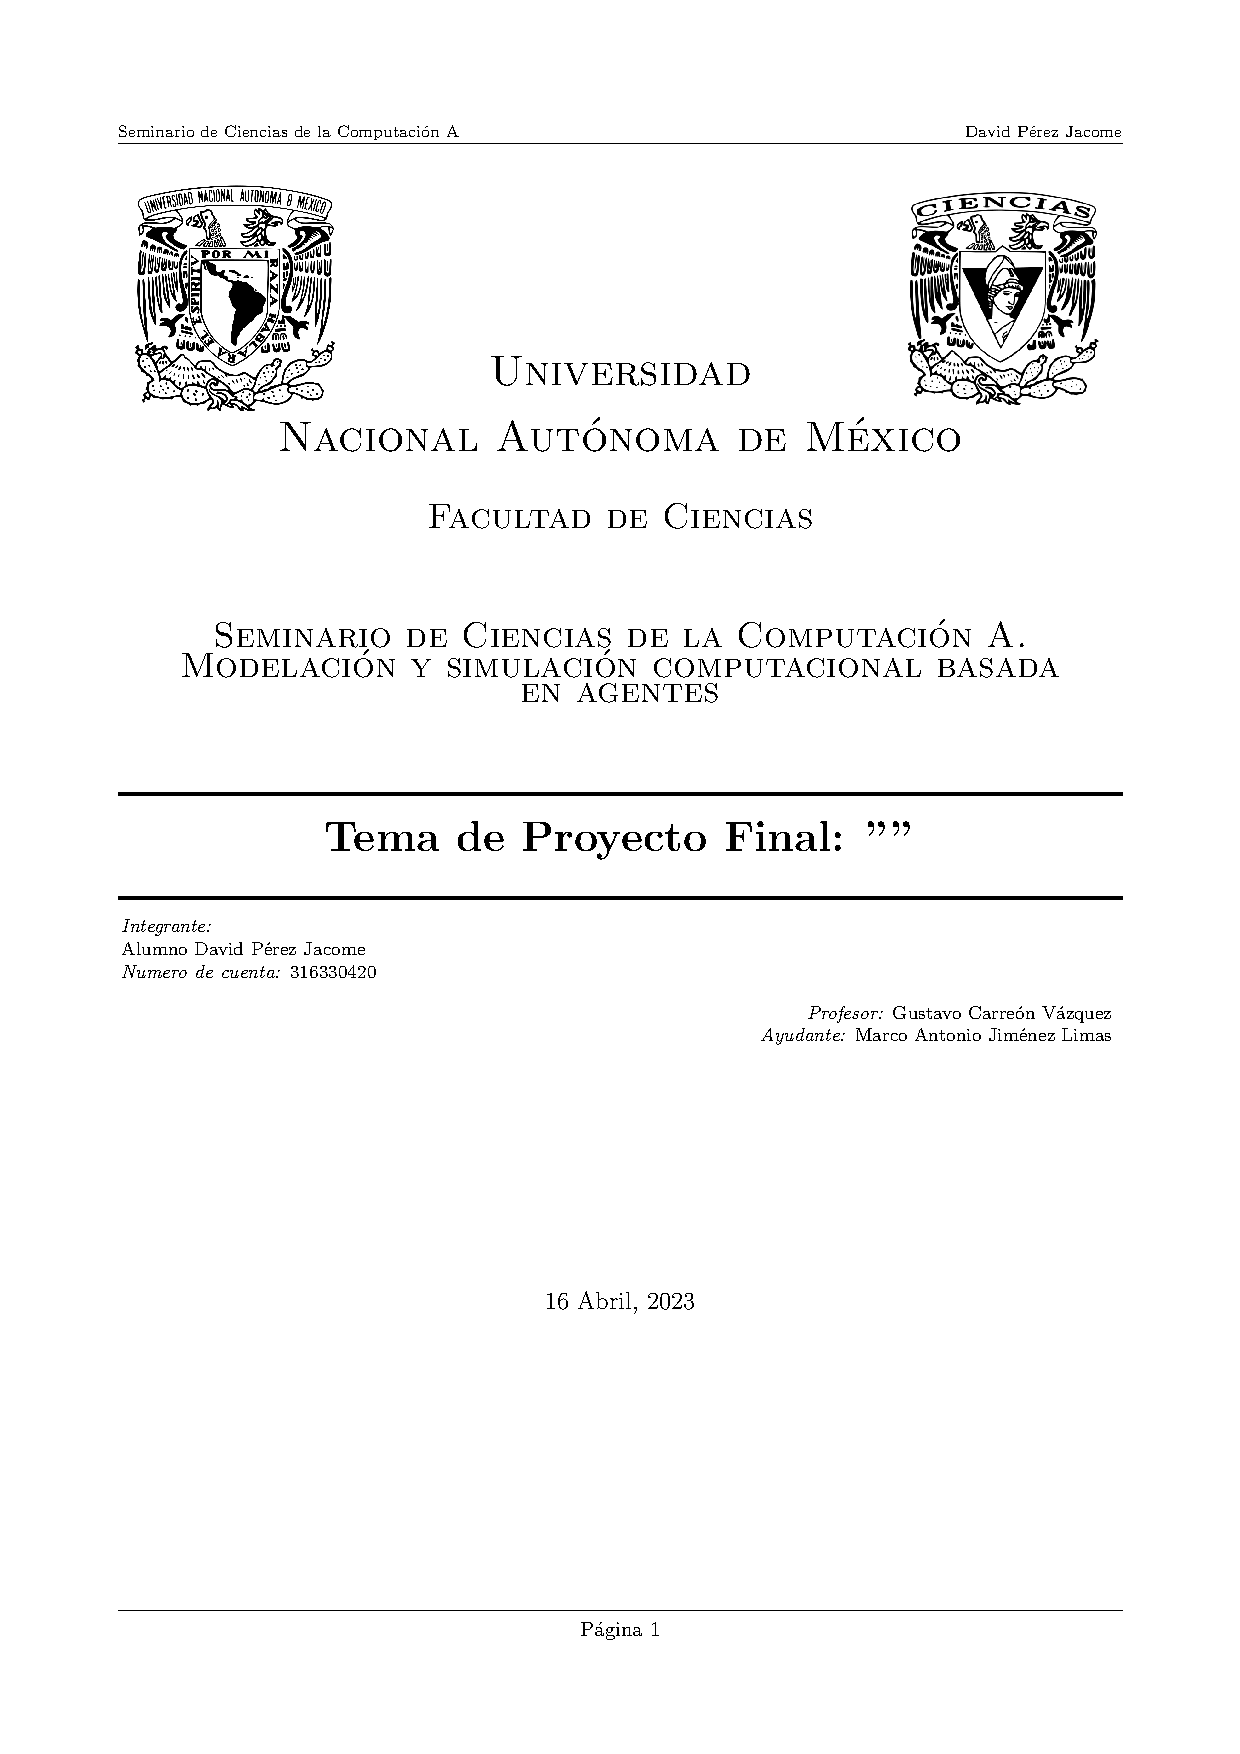
\includepdf{Portada.pdf}
{\color{red} \section*{Practica 2: Tema de Proyecto Final.}}

%Presentacion.pdf: Es el planteamiento e información para su proyecto
%final: debe contener: tema, objetivo, descripción del modelo y
%bibliografía

{\color{blue} \subsection*{Parte 3. Tema de proyecto final }}
\vspace{1em}

A lo largo del curso se han revisado varios sistemas modelados con Autómatas Celulares o Modelación Basada en Agentes.\\

Para realizar el proyecto final deberán escoger un tema de su interés sustentado en publicaciones académicas (libros o artículos) para
cumplir el siguiente objetivo:\\

{\color{red} \section*{Tema: Redes de computadoras: la MBA se puede utilizar para modelar la comunicación y el flujo de datos en redes de computadoras complejas, como Internet.}}

{\color{red} \section*{Objetivo.}}

El objetivo es analizar y modelar en base a lo visto en la materia de Modelación Basada en Agentes, el como se comportan las redes computacionales, flujo de datos via internet.

{\color{red} \section*{Descripción del modelo.}}

Un modelo basado en agentes para la comunicación y el flujo de datos en redes de computadoras podría consistir en agentes que representan diferentes componentes de la red, como routers, switches, servidores, clientes, etc. Estos agentes interactúan entre sí para enviar y recibir paquetes de datos a través de la red.\\

Los agentes pueden tener diferentes atributos y comportamientos, como la capacidad de procesamiento, la velocidad de transmisión, la capacidad de almacenamiento en búfer y la ruta preferida para enviar datos. Además, los agentes pueden interactuar con su entorno, como los cambios en la topología de la red o la congestión en ciertos enlaces.\\

El modelo también podría incluir políticas de enrutamiento y protocolos de comunicación que guíen la forma en que los agentes interactúan entre sí y con el entorno. Por ejemplo, se podrían utilizar protocolos de enrutamiento como OSPF o BGP para determinar la mejor ruta para enviar paquetes de datos a través de la red.\\

Una vez que se haya definido el modelo, se podrían realizar simulaciones para analizar el comportamiento de la red en diferentes escenarios, como la carga de tráfico pesada o la falla de un enlace importante. Esto permitiría a los diseñadores de redes optimizar la topología de la red y las políticas de enrutamiento para mejorar su desempeño y confiabilidad.\\





{\color{red} \section*{Bibliografia.}}

\textbf{"Multi-Agent Systems: Algorithmic, Game-Theoretic, and Logical Foundations" de Yoav Shoham y Kevin Leyton-Brown, "Multiagent Systems: A Modern Approach to Distributed Artificial Intelligence" de Gerhard Weiss, y "Agent-Based Modeling and Simulation" de Charles Macal y Michael North.}



\end{document}